\documentclass{article}
\usepackage{amsmath}
\usepackage{amssymb}
\usepackage[a4paper, top=25mm, bottom=25mm, left=25mm, right=25mm]{geometry}
\usepackage{pgfplots}
\usepackage{mathtools}
\usepgfplotslibrary{fillbetween}
\pgfplotsset{compat=1.18}

\begin{document}
\pagestyle{empty}
\large

\begin{center}
2020-2021 Fall \\MAT123 Final\\(18/01/2021)
\end{center}

\noindent 1. Consider the region $R$ bounded by the curve $y=x^3$, and the straight lines $y=-x$ and $y=x+6$.

\hfill

\noindent (i) Write down the integral corresponding to the area of $R$ with respect to $x$.

\hfill

\noindent (ii) Write down the integral corresponding to the area of $R$ with respect to $y$.

\hfill

\noindent 2. Consider the solid $S$ obtained by revolving the region in the first quadrant bounded by $x=-y^2+1,\:y^2=x$ and $y=1/2$ about $x=-1$.

\hfill

\noindent (i) Using the Shell Method, write down the integral corresponding to the volume of the solid $S$.

\hfill

\noindent (ii) Using the Washer Method, write down the integral corresponding to the volume of the solid $S$.

\hfill

\noindent 3. Evaluate the following integrals.

\hfill

\noindent (a) $\displaystyle\int\frac{dx}{x^{2/3}\left(\sqrt[3]{x}+4\right)}$

\hfill

\hfill

\noindent (b) $\displaystyle\int(\ln x)^2\,dx$

\hfill

\hfill

\noindent (c) $\displaystyle\int\frac{dx}{\sqrt{3+x^2}}$

\hfill

\hfill

\noindent (d) $\displaystyle\int\frac{dx}{2+\sin x}$

\hfill

\hfill

\noindent 4. Using the Monotone Convergence Theorem, show that the sequence  $\displaystyle\left(\frac{n^2+1}{n^3}\right)_{n\in\mathbb{N}}$ is convergent.

\hfill

\noindent 5. Use the Integral Test to determine whether the series $\displaystyle\sum_{k=1}^{\infty}\frac1{k^4+k^2}$ converges or diverges.

\hfill

\hfill

\noindent 6. Find the convergence set for the power series  $\displaystyle\sum_{k=1}^\infty\frac{(x+1)^k}{2k}.$

\hfill

\hfill

\noindent 7. Using a Maclaurin series, show that $\displaystyle\lim_{x\to0}\frac{\sin x}x=1$.

\newpage

\begin{center}
2020-2021 Fall Final (18/01/2021) Solutions\\
(Last update: 8/16/25 (16th of August) 3:00 PM)
\end{center}

\noindent 1.
\begin{center}
\begin{minipage}{0.45\linewidth}
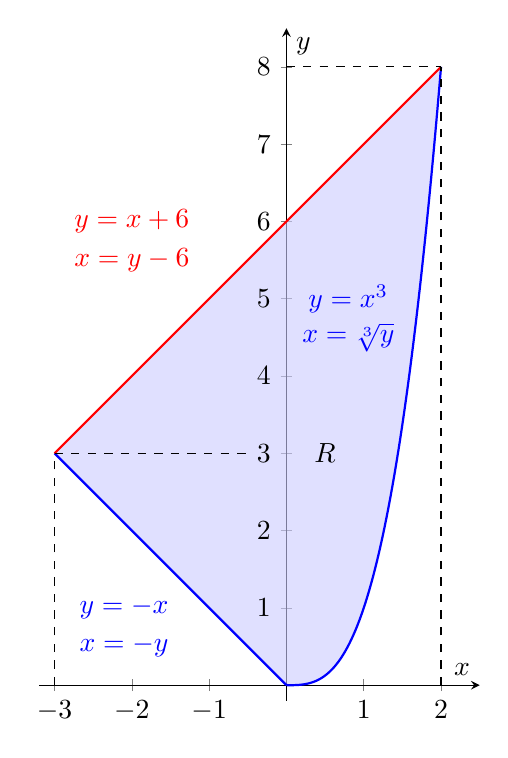
\begin{tikzpicture}
  \begin{axis}[
      axis lines=center,
      axis equal image,
      xlabel={$x$},
      ylabel={$y$},
      xmin=-3.2, xmax=2.5,
      ymin=-0.2, ymax=8.5,
      samples=200,
      scale=1.5,
      domain=-3:2,
    ]

    \addplot [thick, blue, name path=A, domain=-3:2] {max(-x,x^3)};
    \addplot [thick, red, name path=B, domain=-3:2] {x+6};
    \addplot [blue!20, fill opacity=0.6] fill between[of=A and B,soft clip={domain=-3:2}];
    
    \draw[dashed] (-3,0) -- (-3,3); \draw[dashed] (-3,3) -- (-0.5,3);
    \draw[dashed] (2,0) -- (2,8); \draw[dashed] (0,8) -- (2,8);

    \node[red] at (-2,6) {$y=x+6$}; \node[red] at (-2,5.5) {$x=y-6$};
    \node[blue] at (0.8,5) {$y=x^3$}; \node[blue] at (0.8,4.5) {$x=\sqrt[3]{y}$};
    \node[blue] at (-2.1,1) {$y=-x$}; \node[blue] at (-2.1,0.5) {$x=-y$};
    \node at (0.5,3) {$R$};
\end{axis}
\end{tikzpicture}
\end{minipage}\begin{minipage}{0.5\linewidth}
\[\begin{array}{rc}
\text{(i)}&\boxed{\begin{array}{l}\displaystyle\int_{-3}^0\left[(x+6)-(-x)\right]\,dx\\\\\displaystyle+\int_0^2\left[(x+6)-\left(x^3\right)\right]\,dx\end{array}}\\\\\\
\text{(ii)}&\boxed{\begin{array}{l}\displaystyle\int_0^3\left[\left(\sqrt[3]{y}\right)-\left(-y\right)\right]\,dy\\\\\displaystyle+\int_3^8\left[\left(\sqrt[3]{y}\right)-\left(y-6\right)\right]\,dy\end{array}}
\end{array}\]
\end{minipage}
\end{center}

\hfill

\noindent 2.
\begin{center}
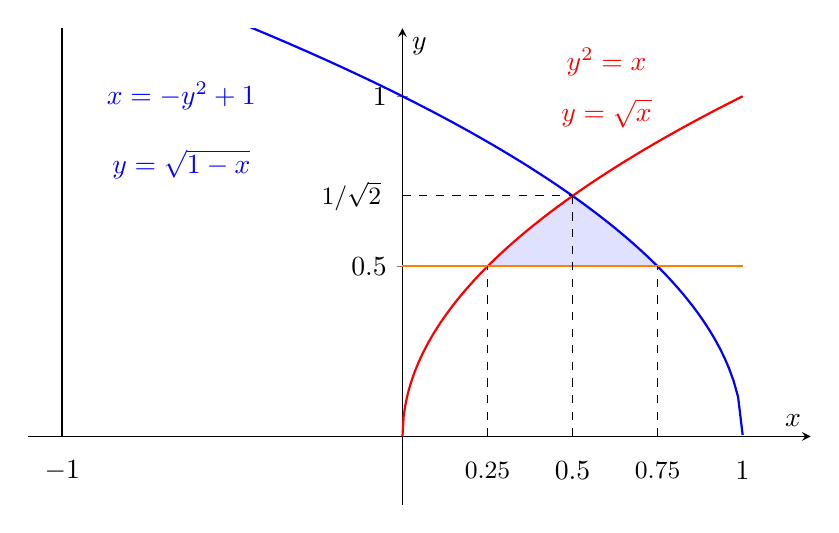
\begin{tikzpicture}
  \begin{axis}[
      axis lines=center,
      axis equal image,
      xlabel={$x$},
      ylabel={$y$},
      xmin=-1.1, xmax=1.2,
      ymin=-0.2, ymax=1.2,
      clip=true,
      scale=1.45,
      xtick=\empty,
    ]

    \addplot [thick, blue, name path=A,samples=150, domain=-1:1] {sqrt(1-x)};
    \addplot [thick, red, name path=B,samples=300, domain=0:1] {sqrt(x)};
    \addplot [thick, orange, name path=C, domain=0:1] {1/2};
    \addplot [blue!20, fill opacity=0.6] fill between[of=B and C,soft clip={domain=0.25:0.5}];
    \addplot [blue!20, fill opacity=0.6] fill between[of=A and C,soft clip={domain=0.5:0.75}];

    \draw[thick] (-1,0)--(-1,2); \draw[dashed] (0.25,0)--(0.25,0.5); \draw[dashed] (0.75,0)--(0.75,0.5); \draw[dashed] (0.5,0)--(0.5,0.707); \draw[dashed] (0,0.707)--(0.5,0.707);
    \node at (0.25,-0.1) {\small$0.25$}; \node at (0.75,-0.1) {\small$0.75$}; \node at (-0.15,0.707) {\small$1/\sqrt2$};

    \node[blue] at (-0.65,1) {$x=-y^2+1$}; \node[blue] at (-0.65,0.8) {$y=\sqrt{1-x}$};
    \node[red] at (0.6,1.1) {$y^2=x$}; \node[red] at (0.6,0.95) {$y=\sqrt{x}$};

    \node at (-1,-0.1) {$-1$}; \node at (1,-0.1) {$1$}; \node at (0.5,-0.1) {$0.5$};
    
  \end{axis}
\end{tikzpicture}
\end{center}

\noindent (i)
\[\boxed{\int_{1/4}^{1/2}2\pi(x+1)\left[\left(\sqrt x\right)-\left(\frac12\right)\right]\,dx+\int_{1/2}^{3/4}2\pi(x+1)\left[\left(\sqrt{1-x}\right)-\left(\frac12\right)\right]\,dx}\]

\hfill

\noindent (ii)
\[\boxed{\int_{1/2}^{1/\sqrt{2}}\pi\left[\left(-y^2+1+1\right)^2-\left(y^2+1\right)^2\right]\,dy}\]

\newpage

\noindent 3.

\hfill

\noindent (a) Let $u=\sqrt[3]{x}+4$, then $du=\dfrac1{3x^{2/3}}\,dx$.

\[\int\frac{dx}{x^{2/3}\left(\sqrt[3]{x}+4\right)}=\int\frac{3du}{u}=3\ln\left|u\right|+c=\boxed{3\ln\left|\sqrt[3]{x}+4\right|+c,\quad c\in\mathbb{R}}\]

\hfill

\noindent (b) Apply integration by parts.

\[\left.\begin{array}{c}
u=(\ln x)^2\implies du=2\ln x\cdot\dfrac1x\,dx\\
dv=dx\implies v=x
\end{array}\right\}\rightarrow \int u\,dv=uv-\int v\,du\]

\[\int(\ln x)^2\,dx=x(\ln x)^2-\int2\ln x\,dx\]

\hfill

\noindent Apply integration by parts once again.

\[\left.\begin{array}{c}
u=\ln x\implies du=\dfrac1x\,dx\\
dv=dx\implies v=x
\end{array}\right\}\rightarrow \int u\,dv=uv-\int v\,du\]

\[\int(\ln x)^2\,dx=x(\ln x)^2-\int2\ln x\,dx\]

\[x(\ln x)^2-\int2\ln x\,dx=x(\ln x)^2-2\left[x\ln x-\int dx\right]=\boxed{x(\ln x)^2-2x\ln x+2x+c,\: c\in\mathbb{R}}\]

\hfill

\noindent (c) Let $x=\sqrt3\tan u$ for $0<u<\dfrac\pi2$, then $dx=\sqrt3\sec^2u\,du$.

\begin{align*}\int\frac{dx}{\sqrt{3+x^2}}&=\int\frac{\sqrt3\sec^2u}{\sqrt{3+3\tan^2u}}\,du=\int\frac{\sec^2u}{\sqrt{1+\tan^2u}}\,du=\int\frac{\sec^2u}{\left|\sec u\right|}\,du\\\\&=\int\sec u\,du\qquad\left[\sec u>0\right]\\\\&=\ln\left|\tan u+\sec u\right|+c,\quad c\in\mathbb{R}\end{align*}

\hfill

\noindent Recall $x=\sqrt3\tan u$.

\[x^2=3\tan^2u=3\sec^2u-3\implies \sec^2u=\frac{x^2+3}3\implies\sec u=\frac{\sqrt{x^2+3}}{\sqrt3}\]

\[\ln\left|\tan u+\sec u\right|+c=\boxed{\ln\left|\frac{x}{\sqrt3}+\frac{\sqrt{x^2+3}}{\sqrt3}\right|+c,\quad c\in\mathbb{R}}\]

\noindent We can omit the constant part.

\[\boxed{\ln\left(x+\sqrt{x^2+3}\right)+c,\quad c\in\mathbb{R}}\]

\hfill

\noindent (d) We may utilize the tangent half-angle substitution, which is also called the Weierstrass substitution. Let $\displaystyle t=\tan\left(\frac x2\right)$. After some mathematical operations, we get the following.

\[\sin x={\frac{2t}{1+t^{2}}},\quad\cos x={\frac{1-t^{2}}{1+t^{2}}},\quad dx={\frac2{1+t^{2}}}\,dt\]

\begin{align*}\int\frac{dx}{2+\sin x}&=\int\frac2{1+t^2}\cdot\frac1{2+\frac{2t}{1+t^2}}\,dt=\int\frac{dt}{t^2+t+1}=\int\frac{dt}{t^2+t+\frac14+\frac34}\\\\&=\int\frac{dt}{\left(t+\frac12\right)^2+\frac34}=\frac43\int\frac{dt}{\frac43\left(t+\frac12\right)^2+1}=\frac43\int\frac{dt}{\left(\frac2{\sqrt3}\right)^2\left(t+\frac12\right)^2+1}\end{align*}

\hfill

\noindent Let $\displaystyle u=\frac2{\sqrt3}\left(t+\frac12\right)$, then $\displaystyle du=\frac2{\sqrt3}\,dt$.

\begin{align*}\frac{2\sqrt3}3\int\frac{du}{u^2+1}&=\frac{2\sqrt3}3\arctan u+c=\frac{2\sqrt3}3\arctan\left(\frac2{\sqrt3}\left(t+\frac12\right)\right)+c\\\\&=\boxed{\frac{2\sqrt3}3\arctan\left(\frac2{\sqrt3}\left(\tan\left(\frac x2\right)+\frac12\right)\right)+c,\quad c\in\mathbb{R}}\end{align*}

\hfill

\noindent 4. Take $f(x)=\dfrac{x^2+1}{x^3}$. We have $f'(x)=-\dfrac{x^2+3}{x^4}<0$ for all $x\geq1$. That means $f$ is decreasing for $x\geq1$. We also have

\[f(1)=2,\quad \lim_{x\to\infty}f(x)=\lim_{x\to\infty}\left(\frac1x +\frac1{x^3}\right)\qquad \implies0<f(x)\leq2,\quad x\geq1\]

\hfill

\noindent Since the sequence is bounded and monotonic, by the Monotone Convergence Theorem, the sequence converges.

\hfill

\noindent 5. Take the corresponding function $\displaystyle f(x)=\frac1{x^4+x^2}$. $f$ is positive for $x\geq1$ because $x^4>0$ and $x^2>0$. $f$ is also continuous for $x\geq1$ because the denominator is a polynomial whose \textit{only} root is zero, which is out of the boundary of the integral. Investigate the monotonicity of $f$ by taking the first derivative.

\[f'(x)=-\frac{4x^3+2x}{\left(x^4+x^2\right)^2}\implies f'(x)\leq0\:\text{for}\:x\geq1\]

\hfill

\noindent We may now apply the Integral Test since the criteria have been satisfied.

\begin{align*}\int_1^{\infty}\frac{dx}{x^4+x^2}&=\int_1^{\infty}\frac{dx}{x^2\left(x^2+1\right)}=\int_1^{\infty}\left(\frac1{x^2}-\frac1{x^2+1}\right)\,dx\\\\&=\lim_{R\to\infty}\int_1^R\left(\frac1{x^2}-\frac1{x^2+1}\right)\,dx=\lim_{R\to\infty}\left[-\frac1x-\arctan x\right]_1^R\\\\&=\lim_{R\to\infty}\left[\left(-\frac1R-\arctan R\right)-\left(-1-\arctan1\right)\right]=1-\frac\pi4\quad\left(\text{convergent}\right)\end{align*}

\hfill

\noindent By the Integral Test, the series $\displaystyle\sum_{k=1}^{\infty}\frac1{k^4+k^2}$ also converges.

\hfill

\noindent 6. Apply the Ratio Test for absolute convergence, and apply other tests at the endpoints.

\[\lim_{n\to\infty}\left|\frac{(x+1)^{k+1}}{2(k+1)}\cdot\frac{2k}{(x+1)^k}\right|=\lim_{n\to\infty}\left|\frac{(x+1)\cdot k}{k+1}\right|=|x+1|\cdot\lim_{n\to\infty}\left|\frac{k}{k+1}\right|=|x+1|\]
\[|x+1|<1\implies-1<x+1<1\implies-2<x<0\quad(\text{convergent})\]

\hfill

\noindent Now, take a look at the endpoints.

\[x=-2\rightarrow\sum_{k=1}^{\infty}\frac{(-1)^k}{2k}=\frac12\sum_{k=1}^{\infty}\frac{(-1)^k}k\]

\hfill

\noindent This is an alternating series. The non-alternating part, which is $\frac1k$, is nonincreasing for $k\geq1$ and it is positive. The limit at infinity is $0$. By Leibniz's Alternating Series Test, the series converges. Try $x=0$.

\[x=0\rightarrow\sum_{k=1}^{\infty}\frac{1^k}{2k}=\frac12\sum_{k=1}^{\infty}\frac1k\]

\hfill

\noindent This is a $p$-series with $p=1$, for which the series diverges by the $p$-series Test.

\hfill

\noindent The convergence set for the power series is

\[\boxed{[-2, 0)}\]

\hfill

\noindent 7. The Maclaurin series of $\sin x$ is

\[\sum_{n=0}^{\infty}\frac{(-1)^nx^{2n+1}}{(2n+1)!}=x-\frac{x^3}{3!}+\frac{x^5}{5!}-\frac{x^7}{7!}+...\]

\hfill

\noindent Rewrite the limit using this expansion.

\[\lim_{x\to0}\frac{\sin x}{x}=\lim_{x\to0}\left[\frac1x\cdot \left(x-\frac{x^3}{3!}+\frac{x^5}{5!}-\frac{x^7}{7!}+...\right)\right]=\lim_{x\to0}\left(1-\frac{x^2}{3!}+\frac{x^4}{5!}-\frac{x^6}{7!}+...\right)=\boxed{1}\]

\hfill

\end{document}